\chapter{Postprocessing and Data Augmentation}

In the previous chapter a \gls{dnn} classifier was found to be the top performing model for the surface classification problem investigated. In this chapter, two improvements to this model are introduced. First, we use a basic data augmentation technique to increase the size of the training data. Then, outlier suppression and detection methods are discussed.

\section{Data Augmentation}

A recurring problem in training \gls{ann}s is that there simply is not enough data \citep{lemley_bazrafkan_corcoran_2017}. Too little data will make a network prone to overfitting, which means that it becomes highly biased to what it has seen in training and will subsequently perform poorly on any validation or test set. In the preceding chapter dropout was introduced for this particular purpose, and examining the cross validation accuracies, it is clear that reasonable accuracy is attained without any further means.

However, by \emph{augmenting} the data we can further increase the training set size, and subsequently further increase model performance. Data augmentation is the process of supplementing a dataset with similar data created from the same dataset. How one augments a dataset is completely dependent on the data. In for instance computer vision, data augmentation often involves rotating, translating, blurring or in some other way modifying existing images \citep{lemley_bazrafkan_corcoran_2017}.

In the present case of increasing the number of smaller data matrices with $T$ slow time samples from a given data matrix with $Q$ slow time samples, we can allow for overlapping batches. Previously, when batches of length $T$ were generated from $Q$ slow time samples, every $T$ sweeps produced one data matrix providing a total of $Q/T$ matrices for analysis. However, noting that any sequence of $T$ radar sweeps is a valid data matrix, we may form \emph{overlapping} matrices from every $T/A$ samples, where $A$ is some integer factor selected so that $T/A$ becomes an integer. This produces $(A-1)(Q/T-1)$ additional matrices providing a total $P$ number of data matrices according to
\begin{equation}
	P = 
	\frac{Q}{T} + (A-1)\Big(\frac{Q}{T} - 1\Big) = 
	\frac{AQ}{T}-A+1.
\end{equation}

Setting $A=5$, one data matrix consisting of 50,000 slow time samples normally yielding 2,000 smaller data matrices with $T=25$ slow time samples, instead produces 9996 matrices. Thus, with this method we are able to increase the number of training data by almost a factor of 5. In table \ref{tab:aug} the effects of data augmentation with $A=5$ is compared to having no augmentation.

% Discuss this result later on.

\begin{table}
	\begin{center}
		\rowcolors{2}{gray!25}{white}
		\begin{tabular}{|c|c|}
			\hline
			\rowcolor{gray!150}
			\color{white}\textbf{A} & \color{white}\textbf{\gls{loo} Acc.} \\
			1 & 98.50 \\
			5 & 98.54 \\
			\hline
		\end{tabular}
	\end{center}
	\caption{Leave-one-out accuracies with and without data augmentation.}
	\label{tab:aug}
\end{table}

%\section{Outlier removal}

%In any dataset some data corruption is to be expected. A grassy surface may have small patches of soil without grass, the device may have been moving at either a too high or too low velocity for a short period of time or the radar sensor iteslf may have had temporary issues. Such processes forms data points inconsistent with the overwhelming bulk of data, or \emph{outliers}, which negatively impacts model performance. The importance of outliers is dependant both of their frequency and magnitude, and can be significantly detrimental to model accuracy making effective removal of them often necessary or at least benifitial \citep{osborne_overbay_2004}, \citep{hodge_austin_2004}. 

\section{Outlier Suppression and Change Detection}

\label{surface_change}
Even with an optimized model with tons of training data, erroneous predictions are inevitable in any real-world scenario. Prediction probabilities are produced by the model rapidly, 8 times a second for a sampling rate of 200 Hz and a batch size $T=25$ according to equation \eqref{eq:classification_rate}. With such errors present in the prediction confidences of the model, what is a reasonable strategy to detect when a change in surface has occurred?  

Many elaborate statistically appealing methods for change detection are presented in \citep{basseville_nikiforov_1993}. These methods require some basic assumptions on the data it attempts to detect a change from, such as for the data having constant probability distribution before and after a parameter change occurs. This, however, renders these methods difficult to use in the present use case, as we are dealing with the output of an artificial neural network producing predictions with unknown structure. This is reinforced by examining what the model outputs, see the top figure in \ref{fig:trans_tgtg}. Predictions remain extremely stable for long periods of time, with occasional outlying predictions every now and then. This makes, as far as we can tell, the methods presented in \citep{basseville_nikiforov_1993} unsuitable for detecting change at the softmax output.

Perhaps most effective way of suppressing data littered with outliers is through some form of median filtering \citep{yin_yang_gabbouj_neuvo_1996}. Median filters are robust against impulsive-type noise, a property that cannot be achieved by traditional linear filtering techniques. The regular form of a median filter simply takes the median of current and previous datapoints, resulting in an output significantly less sensitive to inconsistencies \citep{pearson_2002}. For a sequence $\{p_k\}$ of predictions produced by the \gls{dnn} we apply a median filter of length $L$ and set a decision threshold $\xi$ to produce binary predictions $P_i$ according to \citep{yin_yang_gabbouj_neuvo_1996}
\begin{equation}
	P_i=0 \quad\text{if}\quad\text{median}\{p_k\}_{k=i-L+1}^i\leq\xi, 
	\quad \text{else} \quad P_i = 1
\end{equation}
where $0<\xi<1$. The drawback of using median filtering, or any filtering really, is that the detection is delayed a few predictions. Thus, $L$ must be selected so that the device has not moved too far before the change detection has occurred, but is still capable of sufficiently  suppressing outlying predictions. 


\iffalse
\section{Outlier Supression and Change Detection}


\begin{figure}
	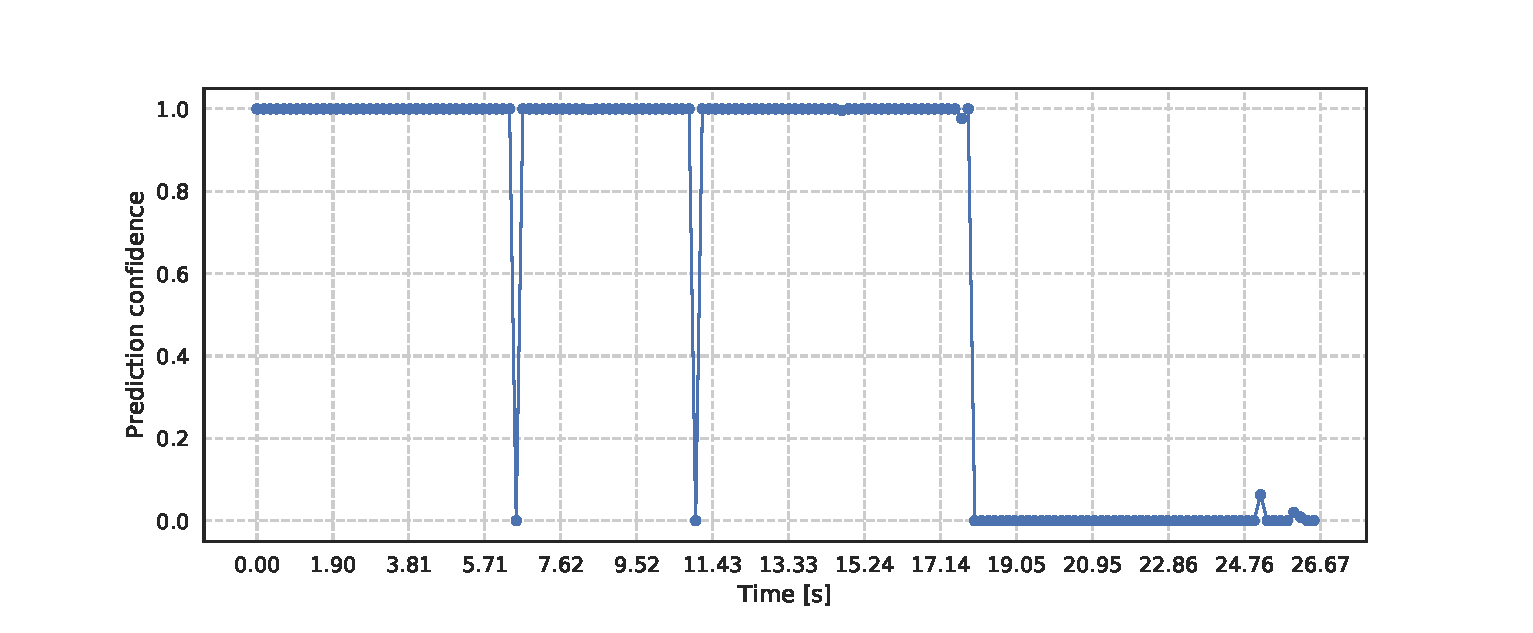
\includegraphics[scale=0.5]{figs_temp/detect_nothing}
	\label{fig:detect_no}
	\caption{Transition region with some outliers}
\end{figure}

\subsection{Thresholding}

The simplest possible detection algorithm is by setting a threshold $\xi$, and classifying below surface as either grass or non-grass depending on whether the prediction is above or below the set threshold. Denoting the resulting prediction as $P$ this detection algorithm is 

\begin{equation}
	P_i=0 \quad\text{if}\quad p_i\leq\xi, \quad
	\text{else} \quad P_i=1
\end{equation}

However, for this method to fail only a single incorrect prediction $p_i$ is required so the algorithm is extremely sensitive to any errors in $p$.

\begin{figure}
	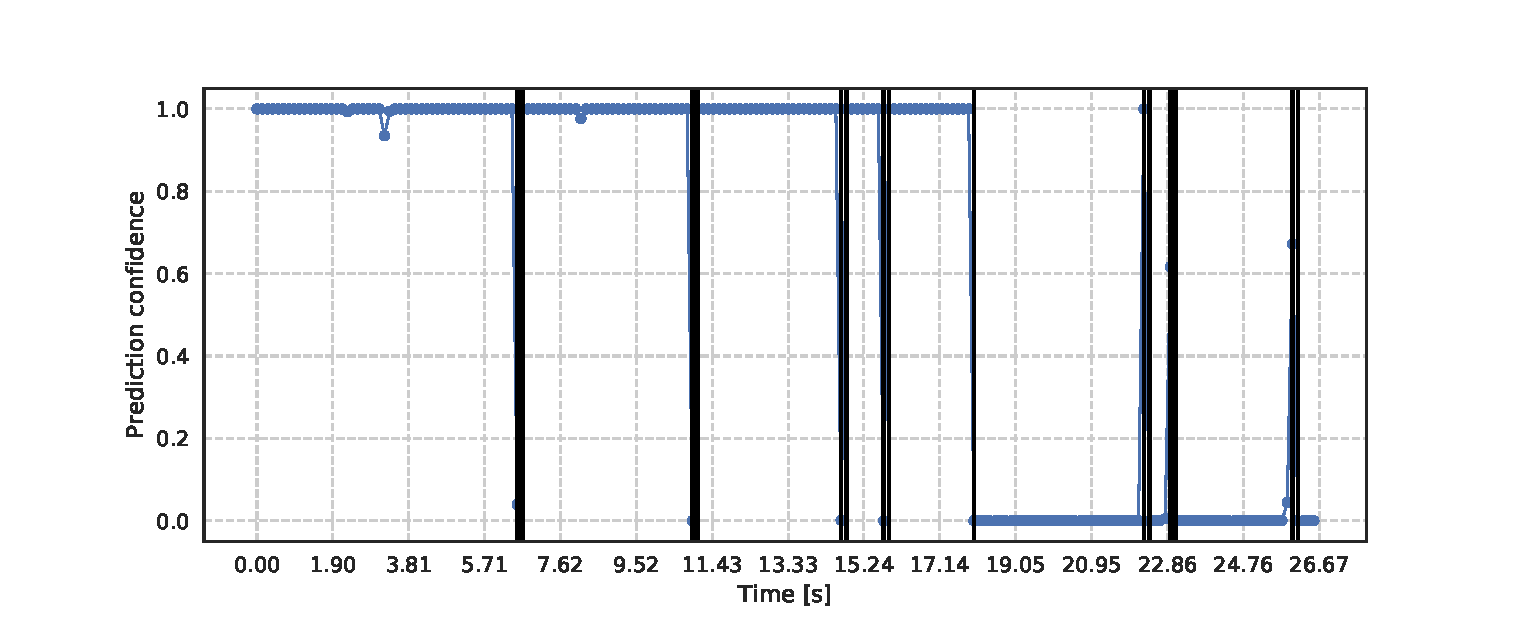
\includegraphics[scale=0.5]{figs_temp/detect_thresh}
	\label{fig:detect_thresh}
	\caption{Detecting transition region using thresholding.}
\end{figure}

\begin{figure}
	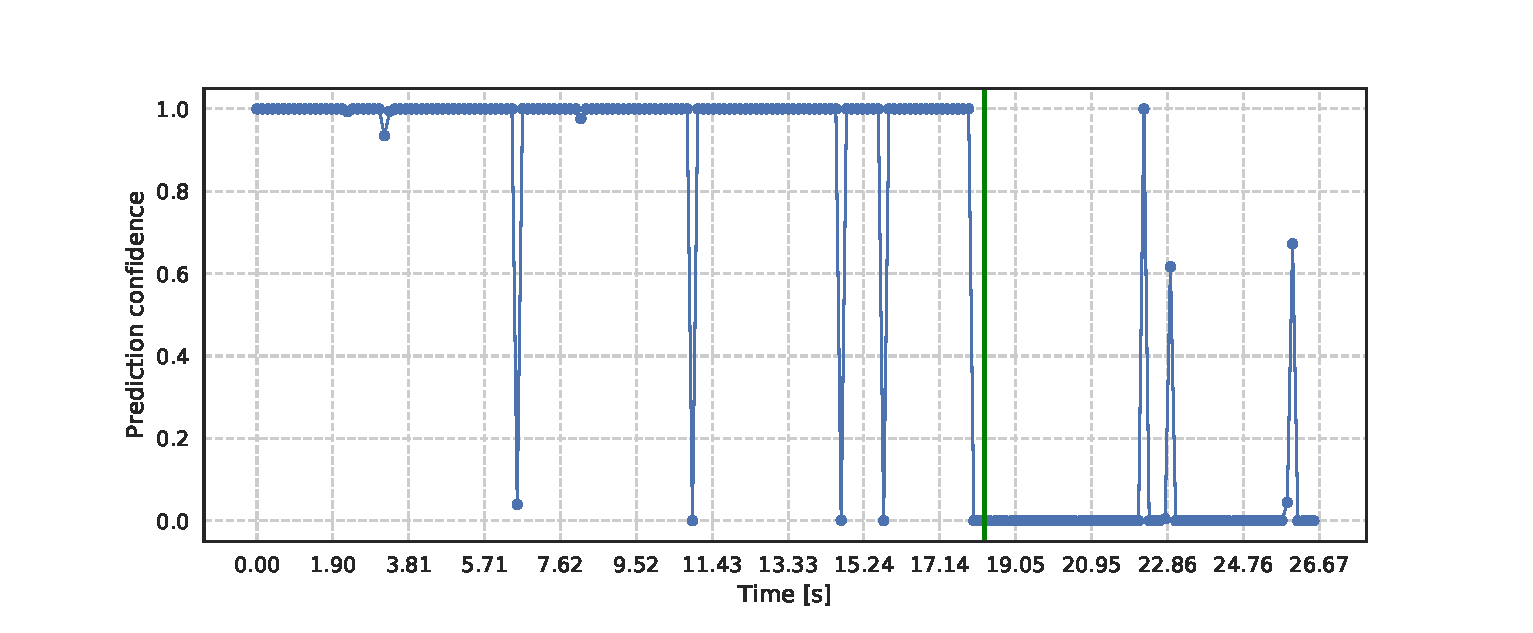
\includegraphics[scale=0.5]{figs_temp/detect_median}
	\label{fig:detect_median}
	\caption{Detection transition using median filtering}
\end{figure}

\subsection{CUSUM}

A traditional and statistically appealing method for effectively detecting abrupt changes in data is CUmulative SUM, hereby refered to as CUSUM. The cumulative sum computed in CUSUM is a log-likelihood $S$ defined through

\begin{equation}
	S_j^k = \sum_{i=j}^k \text{ln}\frac{p_{\theta_1}(y_i)}{p_{\theta_0}(y_i)}
\end{equation}

\begin{figure}
	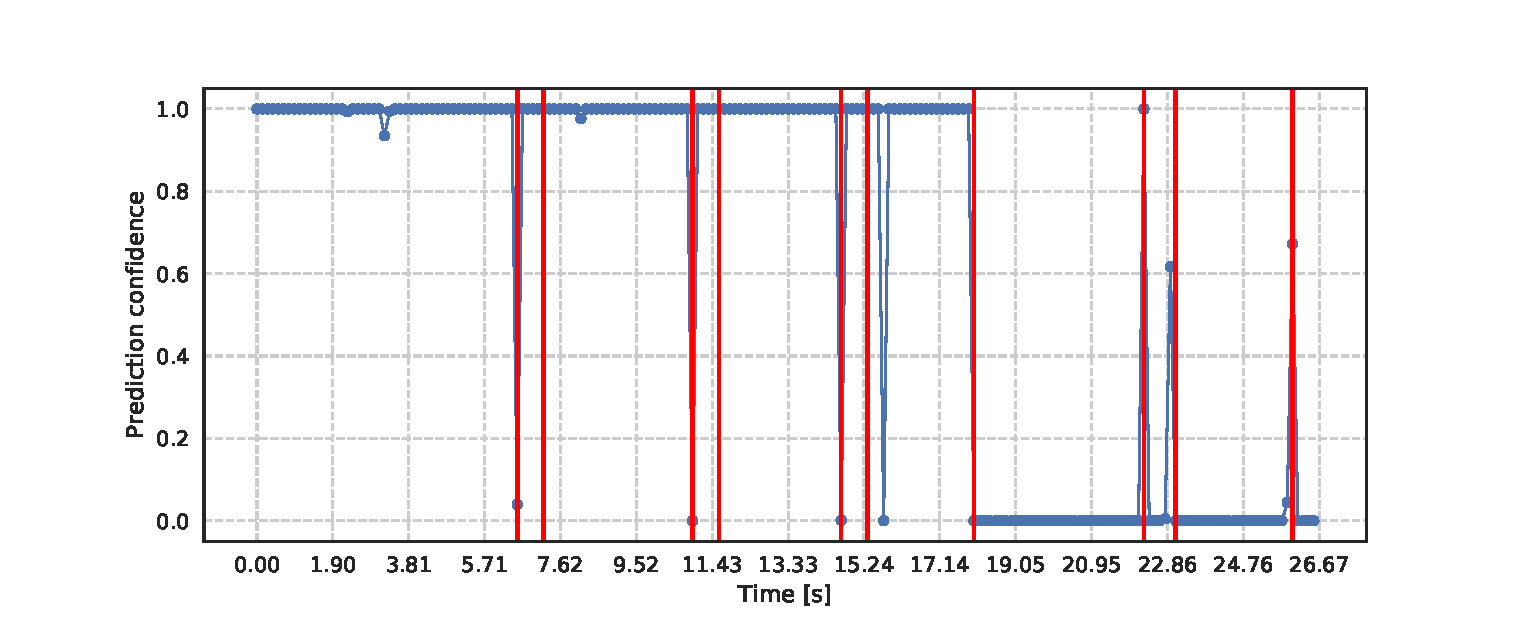
\includegraphics[scale=0.5]{figs_temp/detect_cusum}
	\label{fig:detect_cusum}
	\caption{Detection of transition using CUSUM.}
\end{figure}

[Continue explanation]






\subsection{Method comparison}

After introducing each detection algorithm a comparison is in order. Below is output from a typical transition using [model we made]. Each algorithm has been applied to the data for change detection.


Informal definition as data points inconsistent with our expectations

\section{Removal of outliers}


\subsection{Mahalanobis distance}

\subsection{DBSCAN}

\section{Hyperparameter optimization}
\fi


